\documentclass[11pt]{article}
\usepackage[textwidth=18.0cm, textheight=23.0cm, top=2.0cm]{geometry}
\usepackage{pst-all}
\usepackage{amssymb}
\usepackage{tikz}
\usepackage{underscore}\begin{document}
\pagestyle{empty}


ClassName: \underline{\textbf{Class_07.2bp-22}}
\par
BinSize: \underline{\textbf{100 × 100}}
\par
ReduceSize: \underline{\textbf{100 × 100}}
\par
TypeNum: \underline{\textbf{60}}
\par
Num: \underline{\textbf{60}}
\par
OutS: \underline{\textbf{170000}}
\par
InS: \underline{\textbf{140685}}
\par
Rate: \underline{\textbf{0.828}}
\par
UB: \underline{\textbf{17}}
\par
LB0: \underline{\textbf{17}}
\par
LB: \underline{\textbf{17}}
\par
LBWithCut: \underline{\textbf{17}}
\par
NodeCut: \underline{\textbf{0}}
\par
ExtendedNodeCnt: \underline{\textbf{1}}
\par
GenNodeCnt: \underline{\textbf{1}}
\par
PrimalNode: \underline{\textbf{0}}
\par
ColumnCount: \underline{\textbf{17}}
\par
TotalCutCount: \underline{\textbf{0}}
\par
RootCutCount: \underline{\textbf{0}}
\par
LPSolverCnt: \underline{\textbf{1}}
\par
PricingSolverCnt: \underline{\textbf{0}}
\par
BranchAndBoundNum: \underline{\textbf{1}}
\par
isOpt: \underline{\textbf{true}}
\par
TimeOnInitSolution: \underline{\textbf{600.000 s}}
\par
TimeOnPrimal: \underline{\textbf{0.000 s}}
\par
TimeOnPricing: \underline{\textbf{0.000 s}}
\par
TimeOnRmp: \underline{\textbf{0.078 s}}
\par
TotalTime: \underline{\textbf{600.328 s}}
\par
\newpage


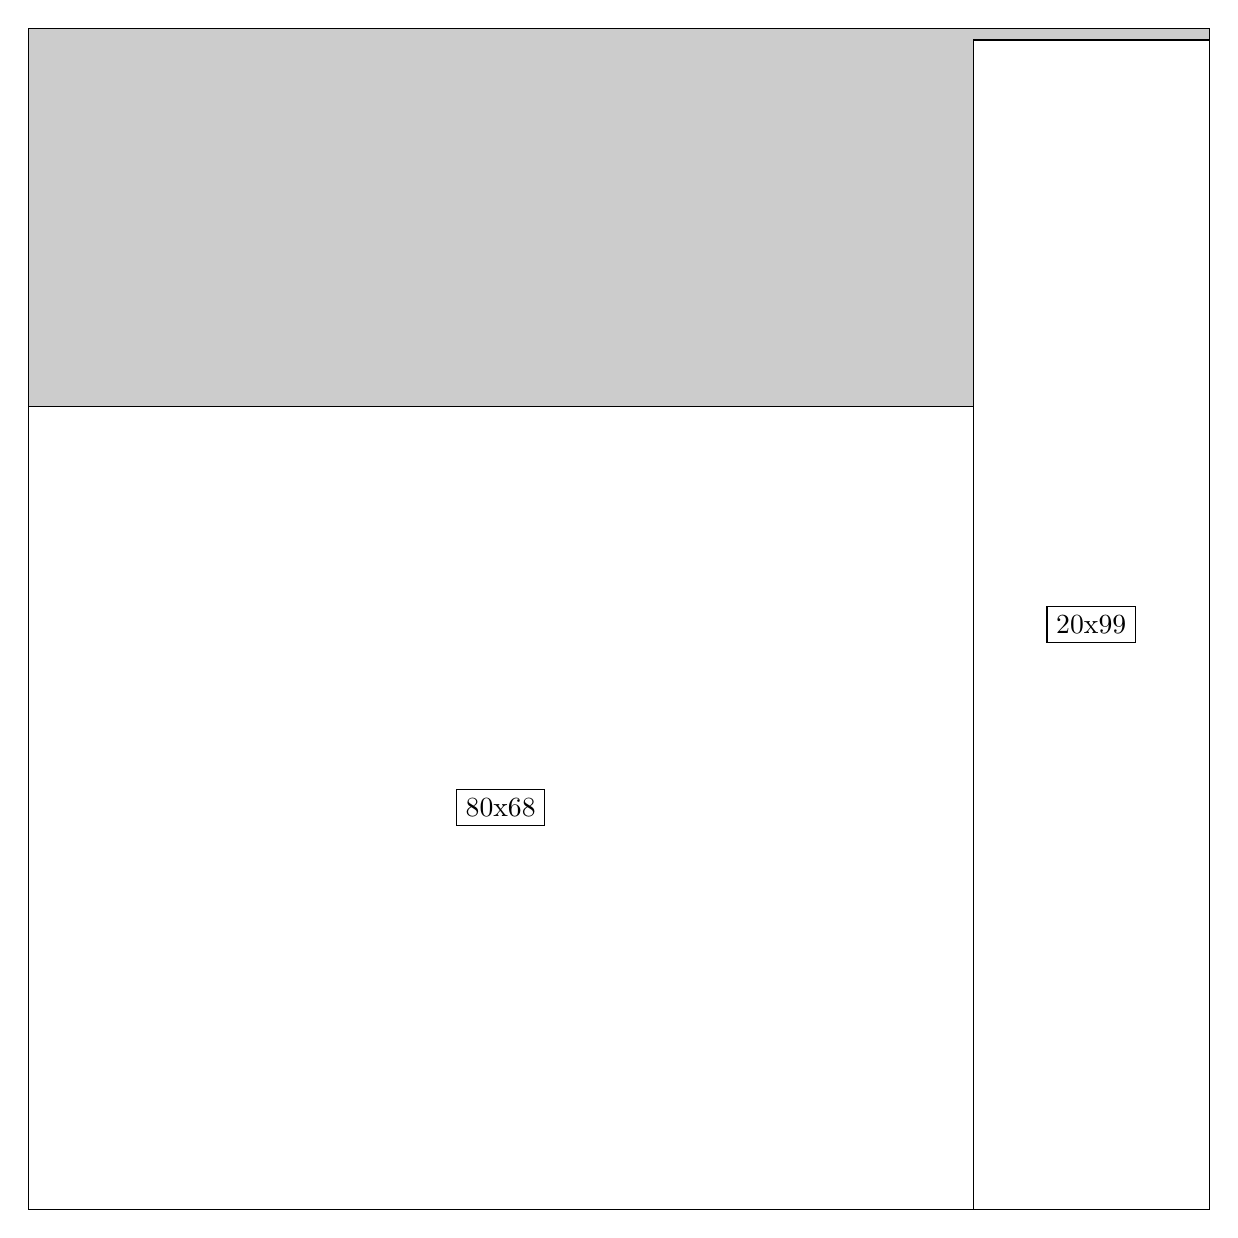
\begin{tikzpicture}[shorten >=1pt,scale=1.0,every node/.style={scale=1.0},->]
\tikzstyle{vertex}=[circle,fill=black!25,minimum size=14pt,inner sep=0pt]
\filldraw[fill=gray!40!white, draw=black] (0,0) rectangle (15.0,15.0);
\foreach \name/\x/\y/\w/\h in {20x99/12.0/0.0/3.0/14.85,80x68/0.0/0.0/12.0/10.2}
\filldraw[fill=white!40!white, draw=black] (\x,\y) rectangle node[draw] (\name) {\name} ++(\w,\h);
\end{tikzpicture}


w =20 , h =99 , x =80 , y =0 , v =1980
\par
w =80 , h =68 , x =0 , y =0 , v =5440
\par
\newpage


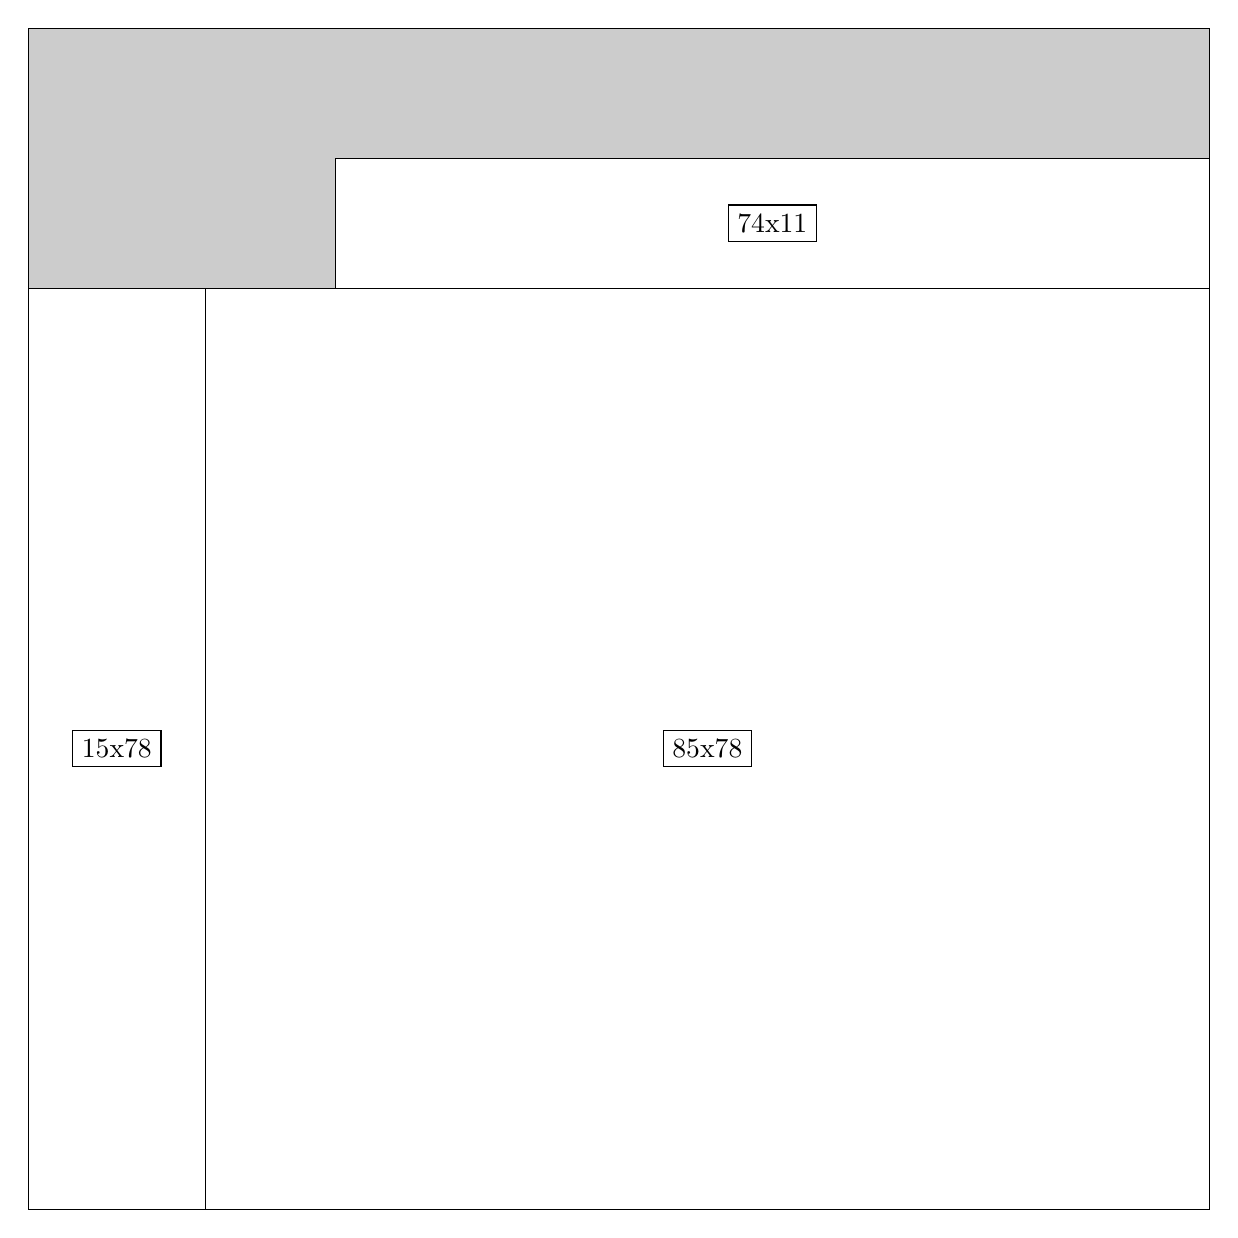
\begin{tikzpicture}[shorten >=1pt,scale=1.0,every node/.style={scale=1.0},->]
\tikzstyle{vertex}=[circle,fill=black!25,minimum size=14pt,inner sep=0pt]
\filldraw[fill=gray!40!white, draw=black] (0,0) rectangle (15.0,15.0);
\foreach \name/\x/\y/\w/\h in {85x78/2.25/0.0/12.75/11.7,74x11/3.9/11.7/11.1/1.65,15x78/0.0/0.0/2.25/11.7}
\filldraw[fill=white!40!white, draw=black] (\x,\y) rectangle node[draw] (\name) {\name} ++(\w,\h);
\end{tikzpicture}


w =85 , h =78 , x =15 , y =0 , v =6630
\par
w =74 , h =11 , x =26 , y =78 , v =814
\par
w =15 , h =78 , x =0 , y =0 , v =1170
\par
\newpage


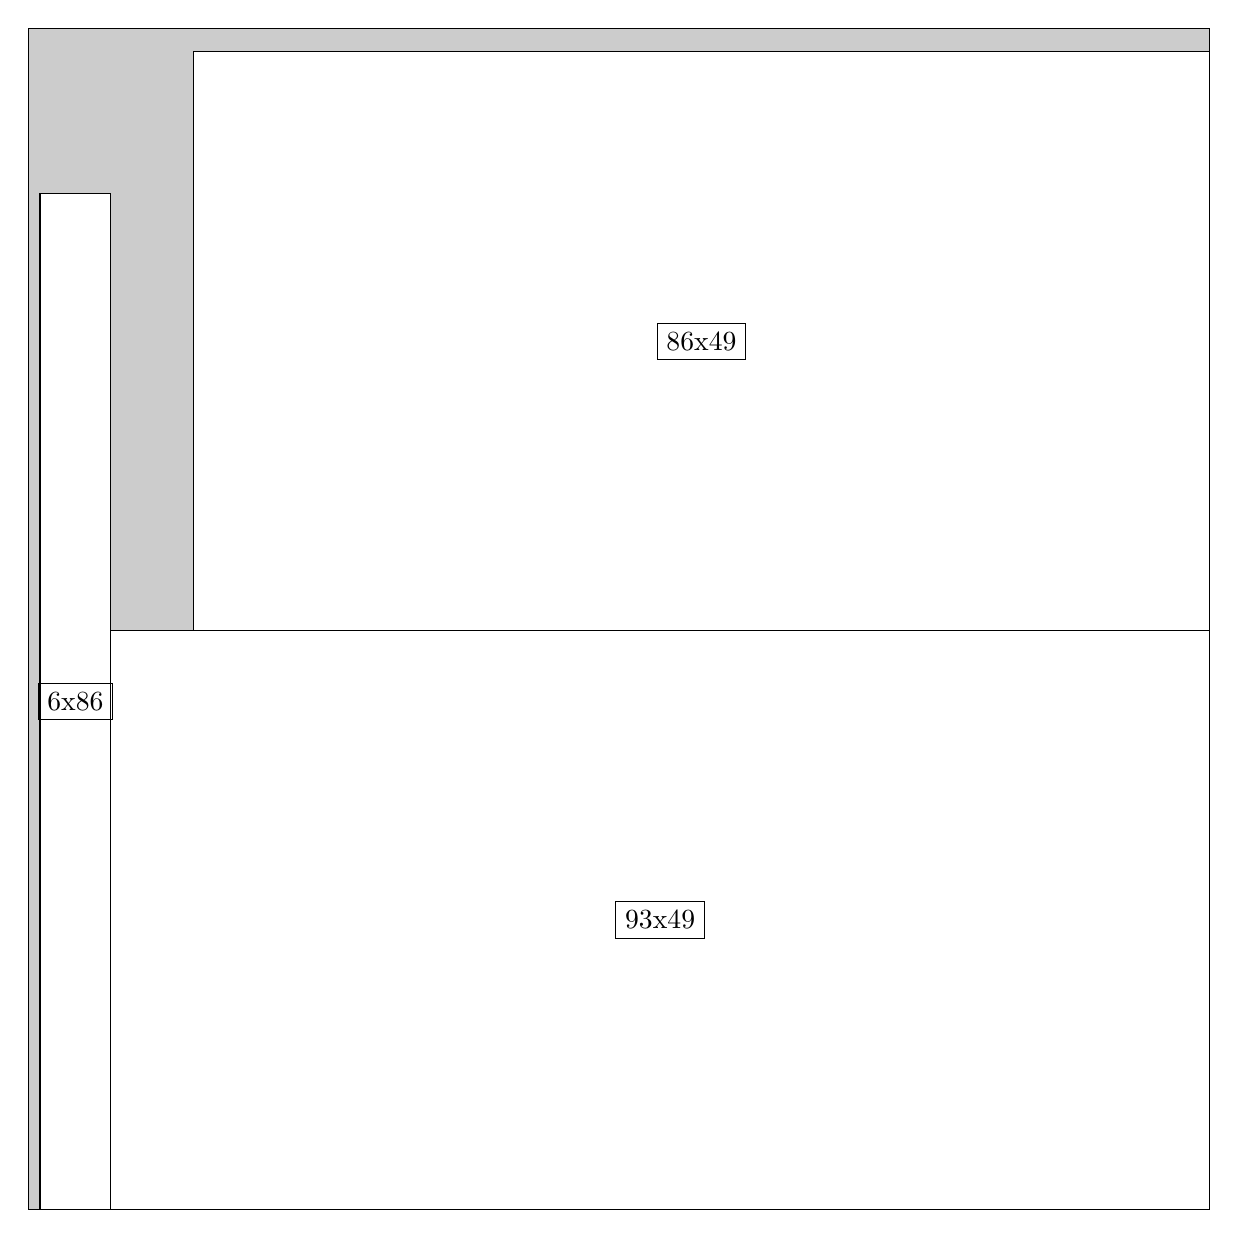
\begin{tikzpicture}[shorten >=1pt,scale=1.0,every node/.style={scale=1.0},->]
\tikzstyle{vertex}=[circle,fill=black!25,minimum size=14pt,inner sep=0pt]
\filldraw[fill=gray!40!white, draw=black] (0,0) rectangle (15.0,15.0);
\foreach \name/\x/\y/\w/\h in {93x49/1.05/0.0/13.95/7.35,86x49/2.1/7.35/12.9/7.35,6x86/0.15/0.0/0.8999999999999999/12.9}
\filldraw[fill=white!40!white, draw=black] (\x,\y) rectangle node[draw] (\name) {\name} ++(\w,\h);
\end{tikzpicture}


w =93 , h =49 , x =7 , y =0 , v =4557
\par
w =86 , h =49 , x =14 , y =49 , v =4214
\par
w =6 , h =86 , x =1 , y =0 , v =516
\par
\newpage


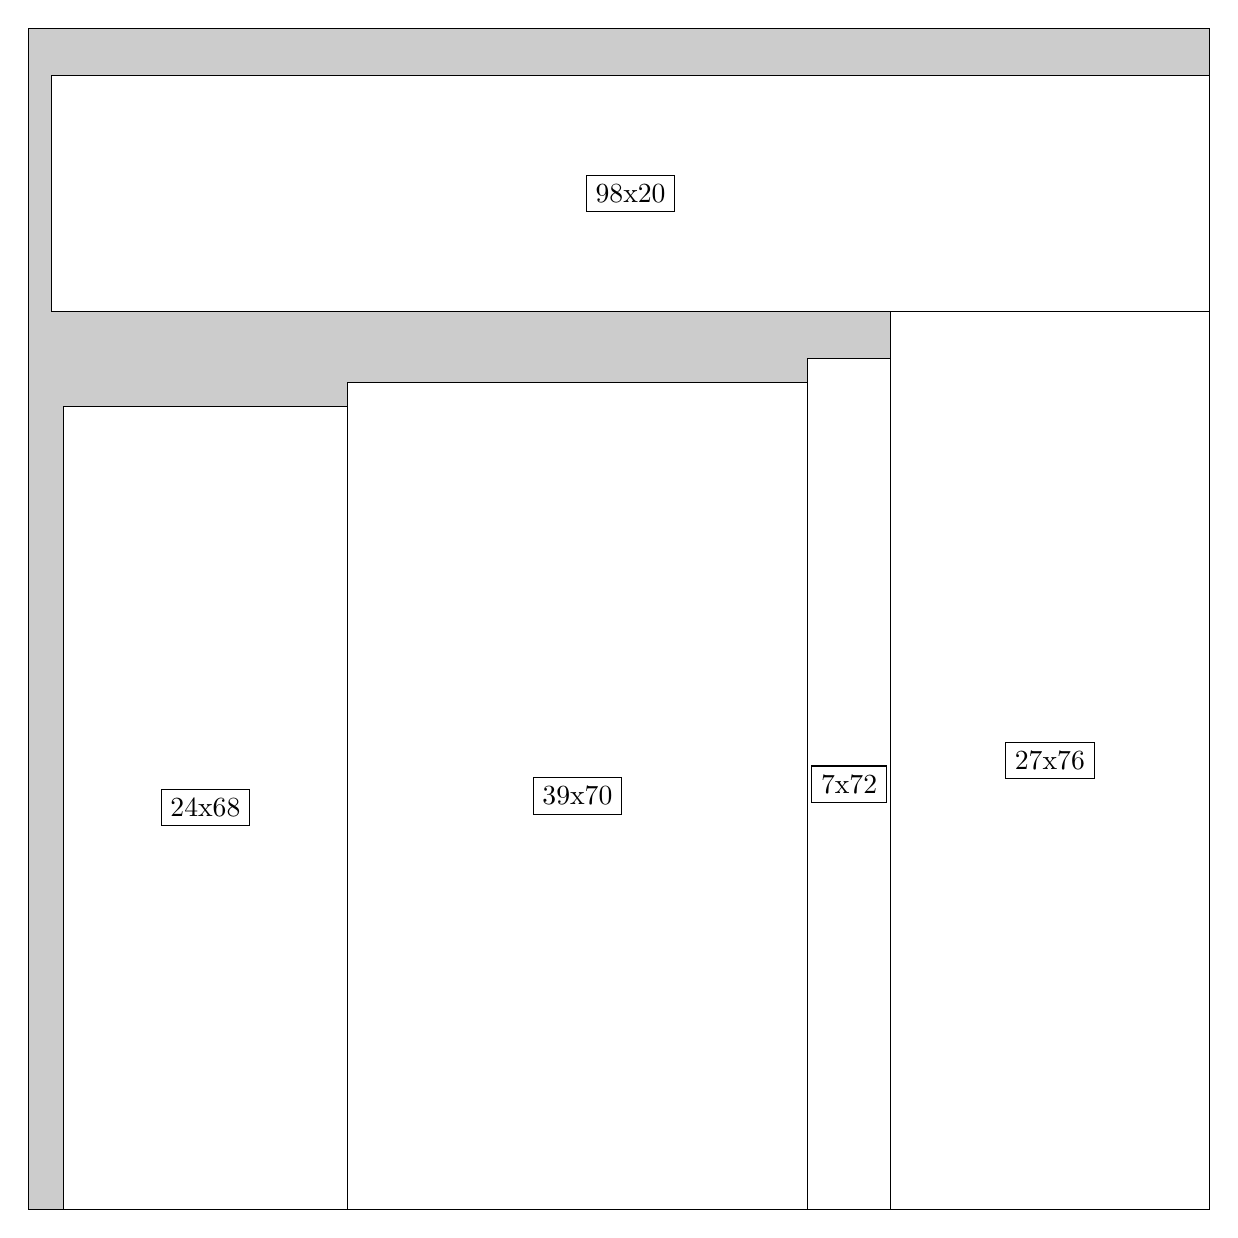
\begin{tikzpicture}[shorten >=1pt,scale=1.0,every node/.style={scale=1.0},->]
\tikzstyle{vertex}=[circle,fill=black!25,minimum size=14pt,inner sep=0pt]
\filldraw[fill=gray!40!white, draw=black] (0,0) rectangle (15.0,15.0);
\foreach \name/\x/\y/\w/\h in {27x76/10.95/0.0/4.05/11.4,7x72/9.9/0.0/1.05/10.799999999999999,39x70/4.05/0.0/5.85/10.5,24x68/0.44999999999999996/0.0/3.5999999999999996/10.2,98x20/0.3/11.4/14.7/3.0}
\filldraw[fill=white!40!white, draw=black] (\x,\y) rectangle node[draw] (\name) {\name} ++(\w,\h);
\end{tikzpicture}


w =27 , h =76 , x =73 , y =0 , v =2052
\par
w =7 , h =72 , x =66 , y =0 , v =504
\par
w =39 , h =70 , x =27 , y =0 , v =2730
\par
w =24 , h =68 , x =3 , y =0 , v =1632
\par
w =98 , h =20 , x =2 , y =76 , v =1960
\par
\newpage


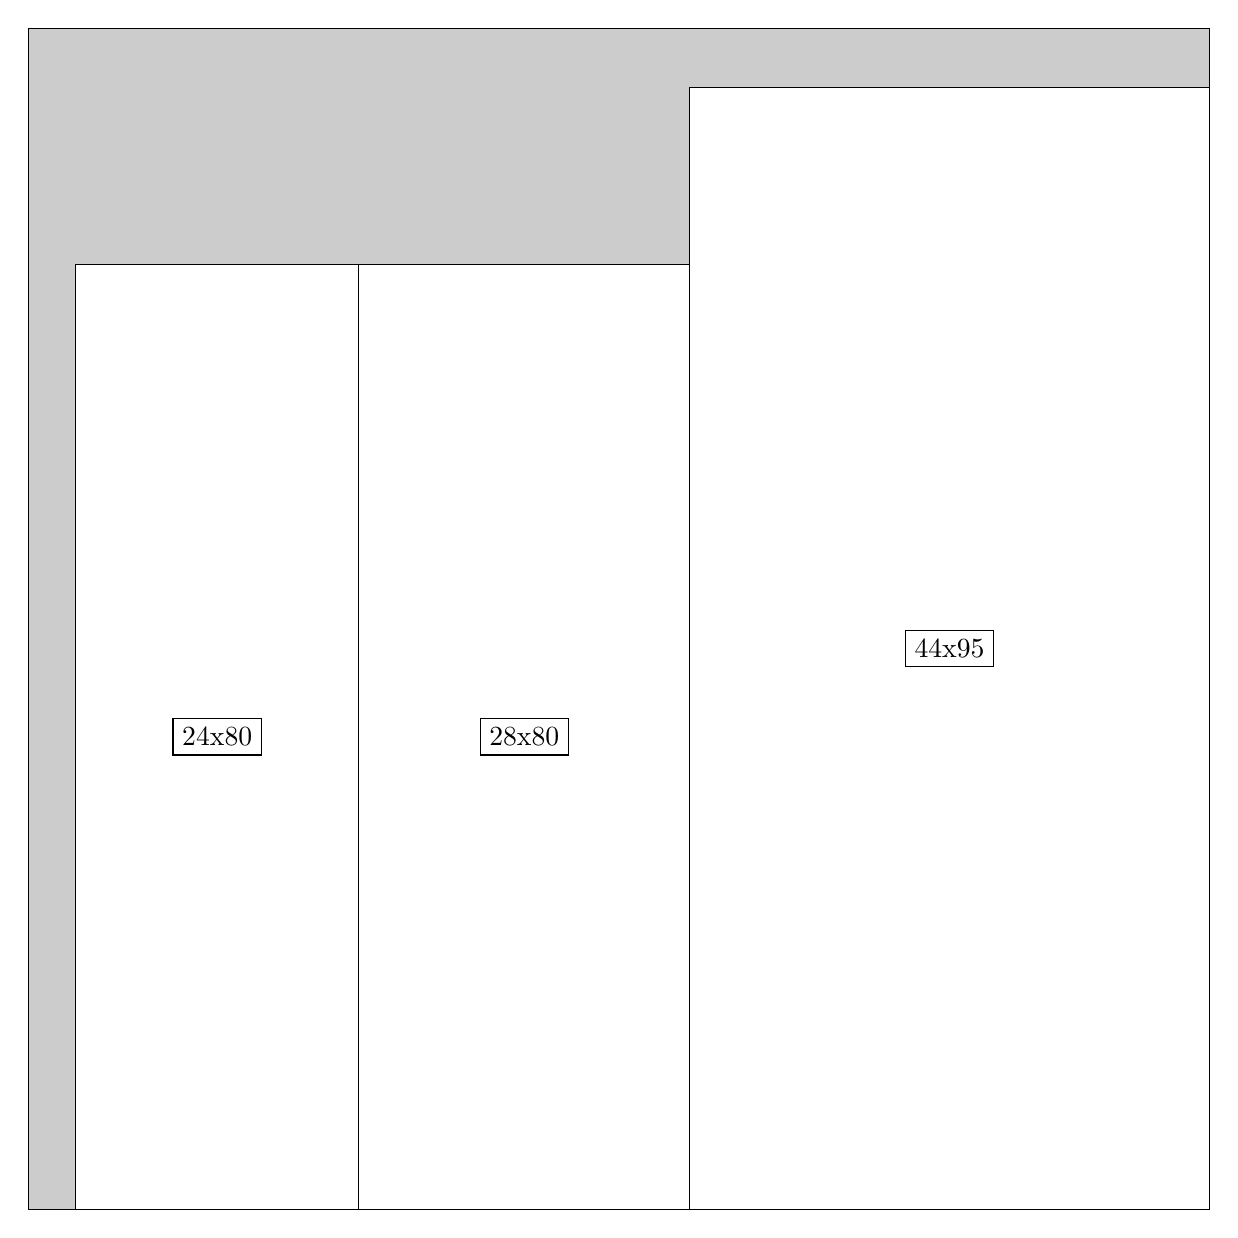
\begin{tikzpicture}[shorten >=1pt,scale=1.0,every node/.style={scale=1.0},->]
\tikzstyle{vertex}=[circle,fill=black!25,minimum size=14pt,inner sep=0pt]
\filldraw[fill=gray!40!white, draw=black] (0,0) rectangle (15.0,15.0);
\foreach \name/\x/\y/\w/\h in {44x95/8.4/0.0/6.6/14.25,28x80/4.2/0.0/4.2/12.0,24x80/0.6/0.0/3.5999999999999996/12.0}
\filldraw[fill=white!40!white, draw=black] (\x,\y) rectangle node[draw] (\name) {\name} ++(\w,\h);
\end{tikzpicture}


w =44 , h =95 , x =56 , y =0 , v =4180
\par
w =28 , h =80 , x =28 , y =0 , v =2240
\par
w =24 , h =80 , x =4 , y =0 , v =1920
\par
\newpage


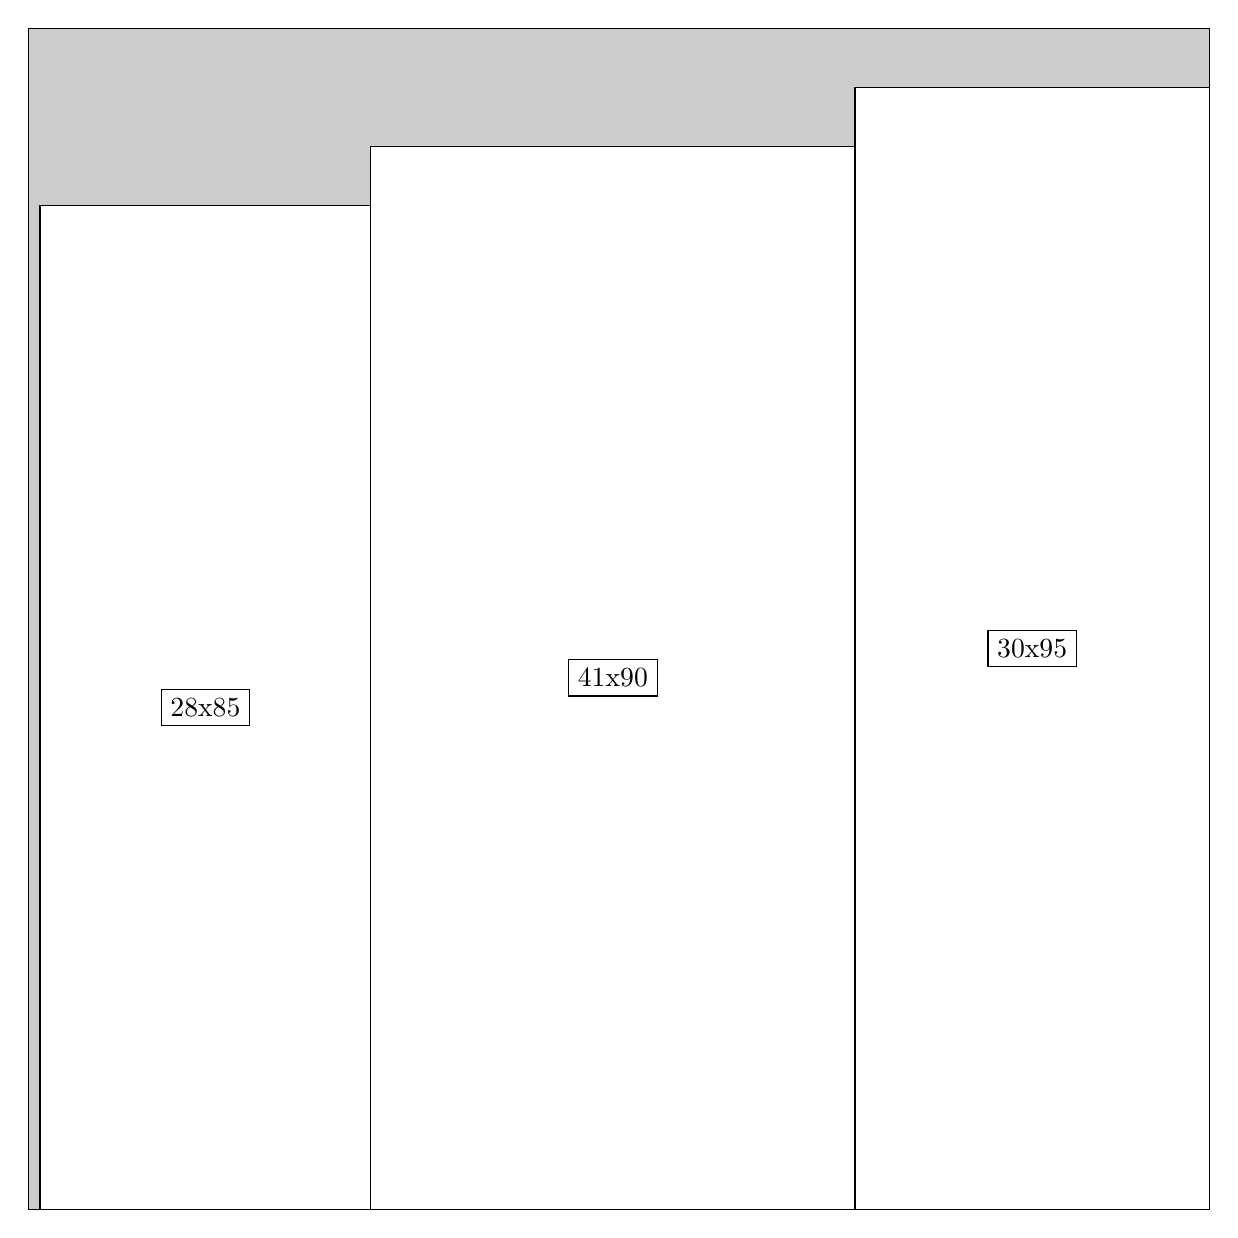
\begin{tikzpicture}[shorten >=1pt,scale=1.0,every node/.style={scale=1.0},->]
\tikzstyle{vertex}=[circle,fill=black!25,minimum size=14pt,inner sep=0pt]
\filldraw[fill=gray!40!white, draw=black] (0,0) rectangle (15.0,15.0);
\foreach \name/\x/\y/\w/\h in {30x95/10.5/0.0/4.5/14.25,41x90/4.35/0.0/6.1499999999999995/13.5,28x85/0.15/0.0/4.2/12.75}
\filldraw[fill=white!40!white, draw=black] (\x,\y) rectangle node[draw] (\name) {\name} ++(\w,\h);
\end{tikzpicture}


w =30 , h =95 , x =70 , y =0 , v =2850
\par
w =41 , h =90 , x =29 , y =0 , v =3690
\par
w =28 , h =85 , x =1 , y =0 , v =2380
\par
\newpage


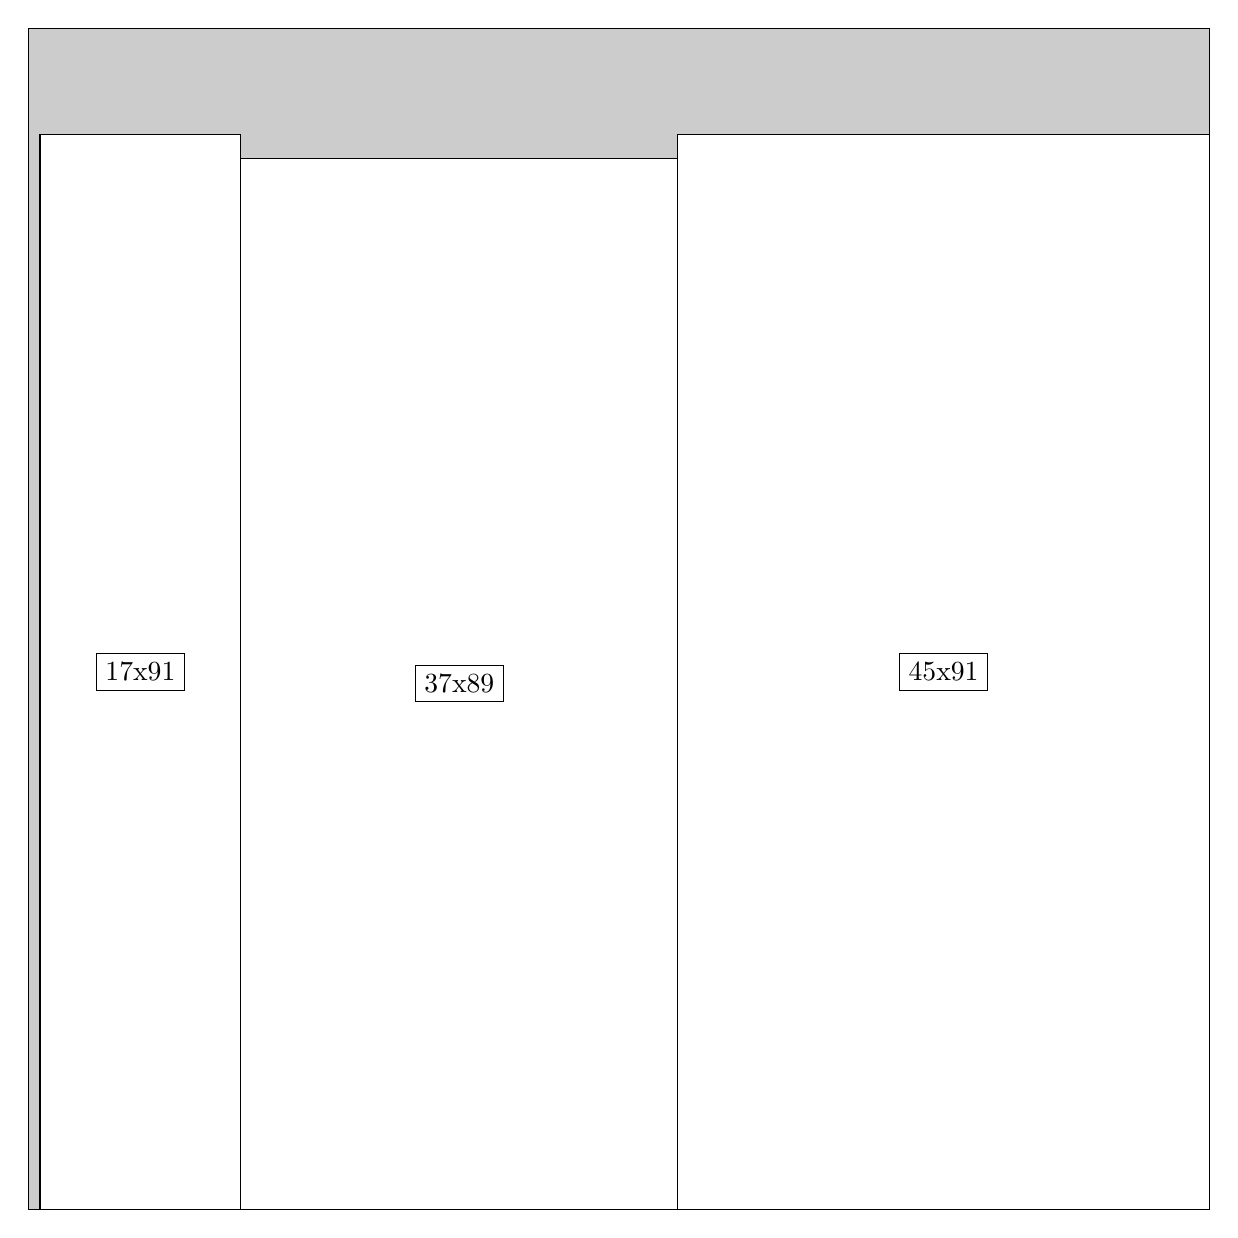
\begin{tikzpicture}[shorten >=1pt,scale=1.0,every node/.style={scale=1.0},->]
\tikzstyle{vertex}=[circle,fill=black!25,minimum size=14pt,inner sep=0pt]
\filldraw[fill=gray!40!white, draw=black] (0,0) rectangle (15.0,15.0);
\foreach \name/\x/\y/\w/\h in {45x91/8.25/0.0/6.75/13.65,37x89/2.6999999999999997/0.0/5.55/13.35,17x91/0.15/0.0/2.55/13.65}
\filldraw[fill=white!40!white, draw=black] (\x,\y) rectangle node[draw] (\name) {\name} ++(\w,\h);
\end{tikzpicture}


w =45 , h =91 , x =55 , y =0 , v =4095
\par
w =37 , h =89 , x =18 , y =0 , v =3293
\par
w =17 , h =91 , x =1 , y =0 , v =1547
\par
\newpage


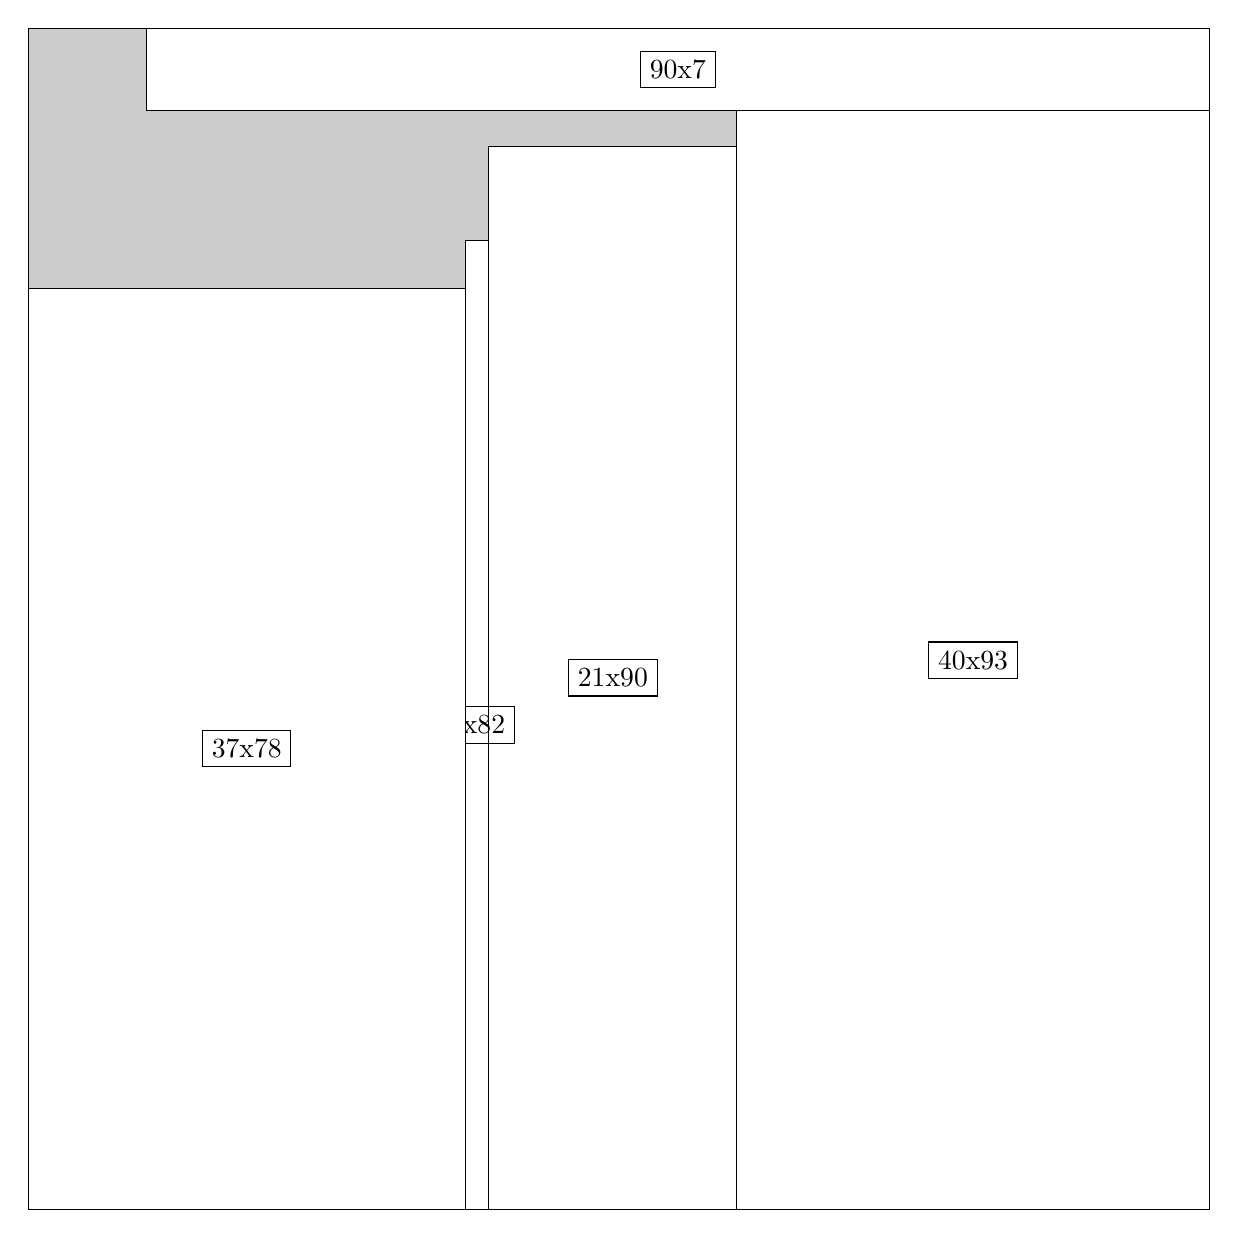
\begin{tikzpicture}[shorten >=1pt,scale=1.0,every node/.style={scale=1.0},->]
\tikzstyle{vertex}=[circle,fill=black!25,minimum size=14pt,inner sep=0pt]
\filldraw[fill=gray!40!white, draw=black] (0,0) rectangle (15.0,15.0);
\foreach \name/\x/\y/\w/\h in {40x93/9.0/0.0/6.0/13.95,21x90/5.85/0.0/3.15/13.5,2x82/5.55/0.0/0.3/12.299999999999999,37x78/0.0/0.0/5.55/11.7,90x7/1.5/13.95/13.5/1.05}
\filldraw[fill=white!40!white, draw=black] (\x,\y) rectangle node[draw] (\name) {\name} ++(\w,\h);
\end{tikzpicture}


w =40 , h =93 , x =60 , y =0 , v =3720
\par
w =21 , h =90 , x =39 , y =0 , v =1890
\par
w =2 , h =82 , x =37 , y =0 , v =164
\par
w =37 , h =78 , x =0 , y =0 , v =2886
\par
w =90 , h =7 , x =10 , y =93 , v =630
\par
\newpage


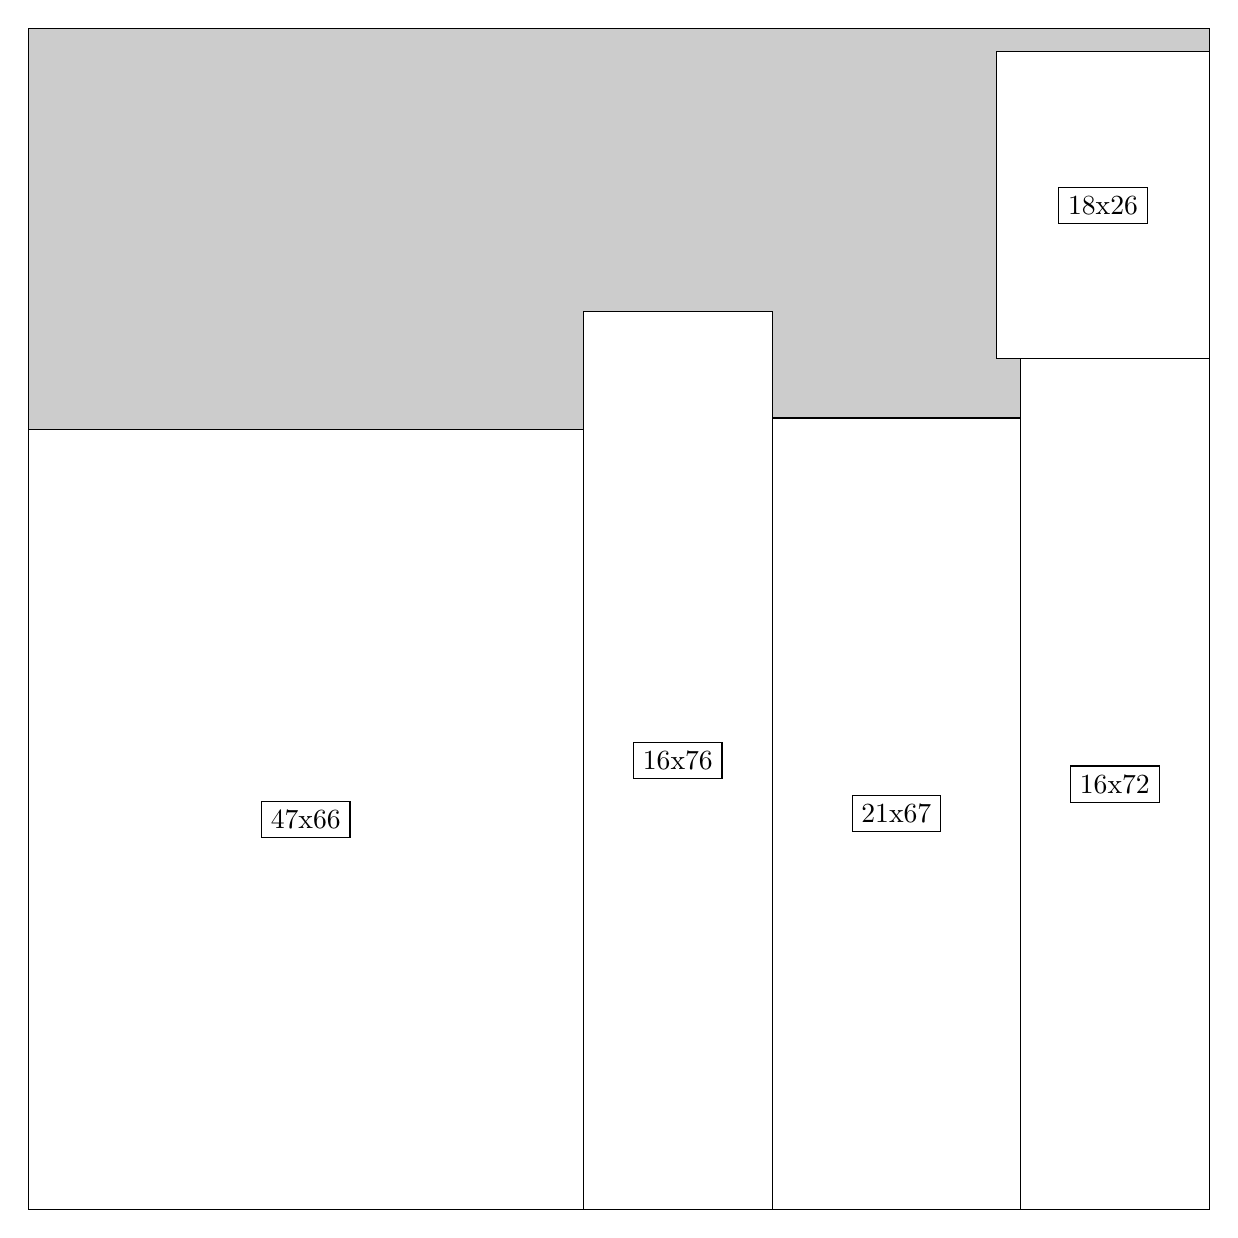
\begin{tikzpicture}[shorten >=1pt,scale=1.0,every node/.style={scale=1.0},->]
\tikzstyle{vertex}=[circle,fill=black!25,minimum size=14pt,inner sep=0pt]
\filldraw[fill=gray!40!white, draw=black] (0,0) rectangle (15.0,15.0);
\foreach \name/\x/\y/\w/\h in {16x72/12.6/0.0/2.4/10.799999999999999,21x67/9.45/0.0/3.15/10.049999999999999,18x26/12.299999999999999/10.799999999999999/2.6999999999999997/3.9,16x76/7.05/0.0/2.4/11.4,47x66/0.0/0.0/7.05/9.9}
\filldraw[fill=white!40!white, draw=black] (\x,\y) rectangle node[draw] (\name) {\name} ++(\w,\h);
\end{tikzpicture}


w =16 , h =72 , x =84 , y =0 , v =1152
\par
w =21 , h =67 , x =63 , y =0 , v =1407
\par
w =18 , h =26 , x =82 , y =72 , v =468
\par
w =16 , h =76 , x =47 , y =0 , v =1216
\par
w =47 , h =66 , x =0 , y =0 , v =3102
\par
\newpage


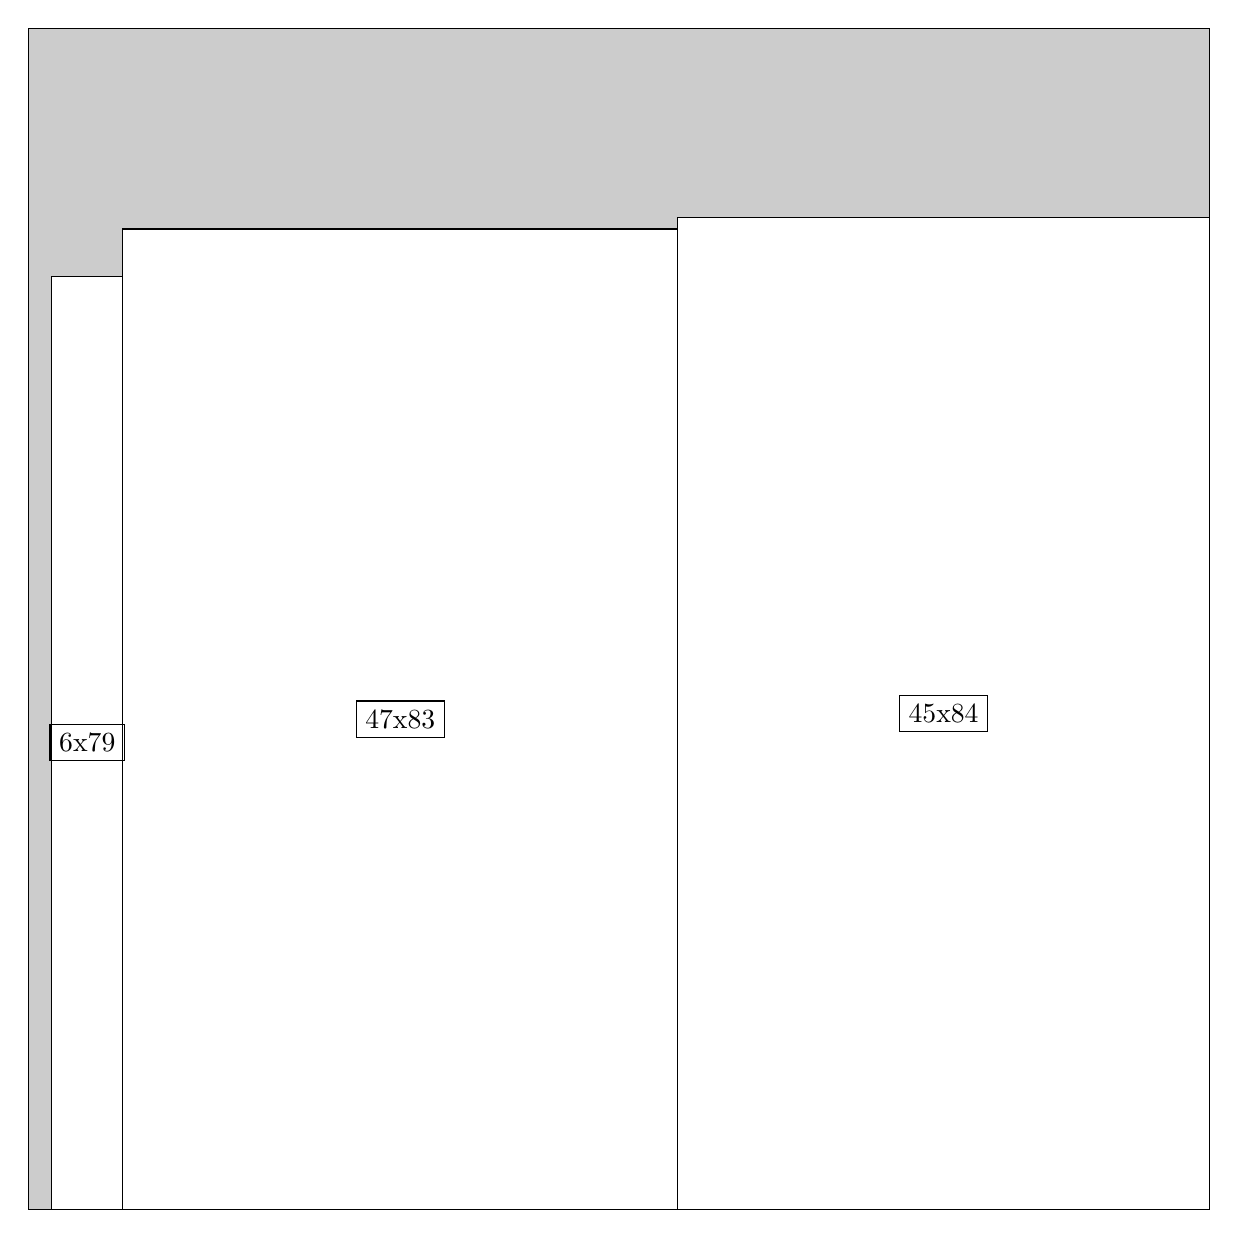
\begin{tikzpicture}[shorten >=1pt,scale=1.0,every node/.style={scale=1.0},->]
\tikzstyle{vertex}=[circle,fill=black!25,minimum size=14pt,inner sep=0pt]
\filldraw[fill=gray!40!white, draw=black] (0,0) rectangle (15.0,15.0);
\foreach \name/\x/\y/\w/\h in {45x84/8.25/0.0/6.75/12.6,47x83/1.2/0.0/7.05/12.45,6x79/0.3/0.0/0.8999999999999999/11.85}
\filldraw[fill=white!40!white, draw=black] (\x,\y) rectangle node[draw] (\name) {\name} ++(\w,\h);
\end{tikzpicture}


w =45 , h =84 , x =55 , y =0 , v =3780
\par
w =47 , h =83 , x =8 , y =0 , v =3901
\par
w =6 , h =79 , x =2 , y =0 , v =474
\par
\newpage


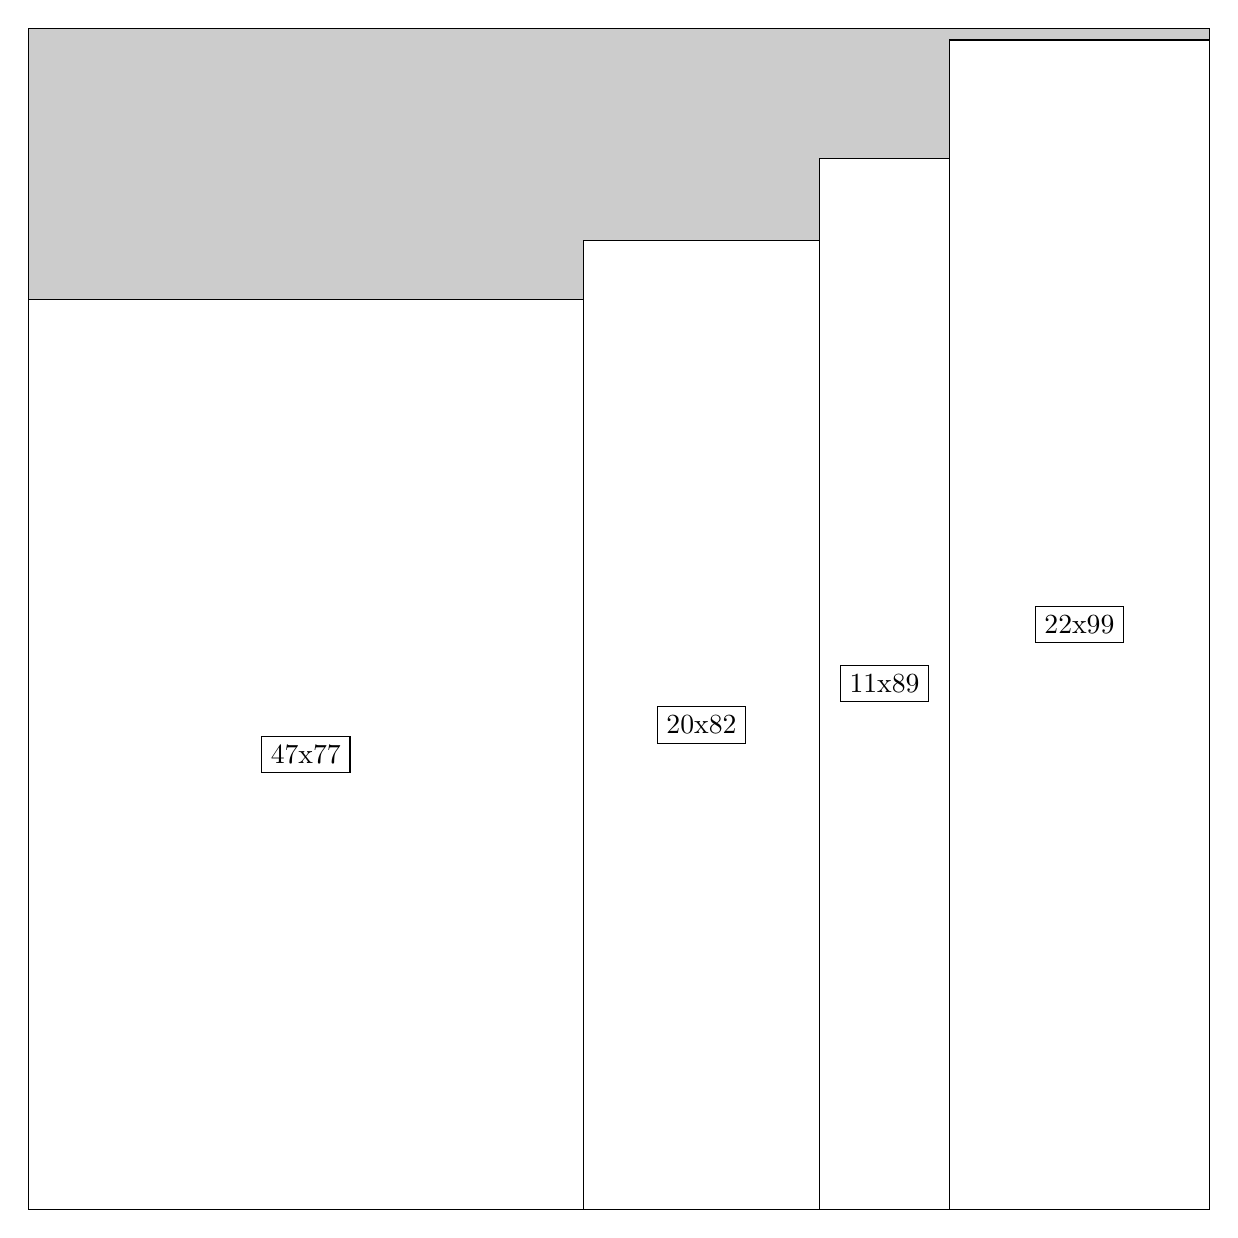
\begin{tikzpicture}[shorten >=1pt,scale=1.0,every node/.style={scale=1.0},->]
\tikzstyle{vertex}=[circle,fill=black!25,minimum size=14pt,inner sep=0pt]
\filldraw[fill=gray!40!white, draw=black] (0,0) rectangle (15.0,15.0);
\foreach \name/\x/\y/\w/\h in {22x99/11.7/0.0/3.3/14.85,11x89/10.049999999999999/0.0/1.65/13.35,20x82/7.05/0.0/3.0/12.299999999999999,47x77/0.0/0.0/7.05/11.549999999999999}
\filldraw[fill=white!40!white, draw=black] (\x,\y) rectangle node[draw] (\name) {\name} ++(\w,\h);
\end{tikzpicture}


w =22 , h =99 , x =78 , y =0 , v =2178
\par
w =11 , h =89 , x =67 , y =0 , v =979
\par
w =20 , h =82 , x =47 , y =0 , v =1640
\par
w =47 , h =77 , x =0 , y =0 , v =3619
\par
\newpage


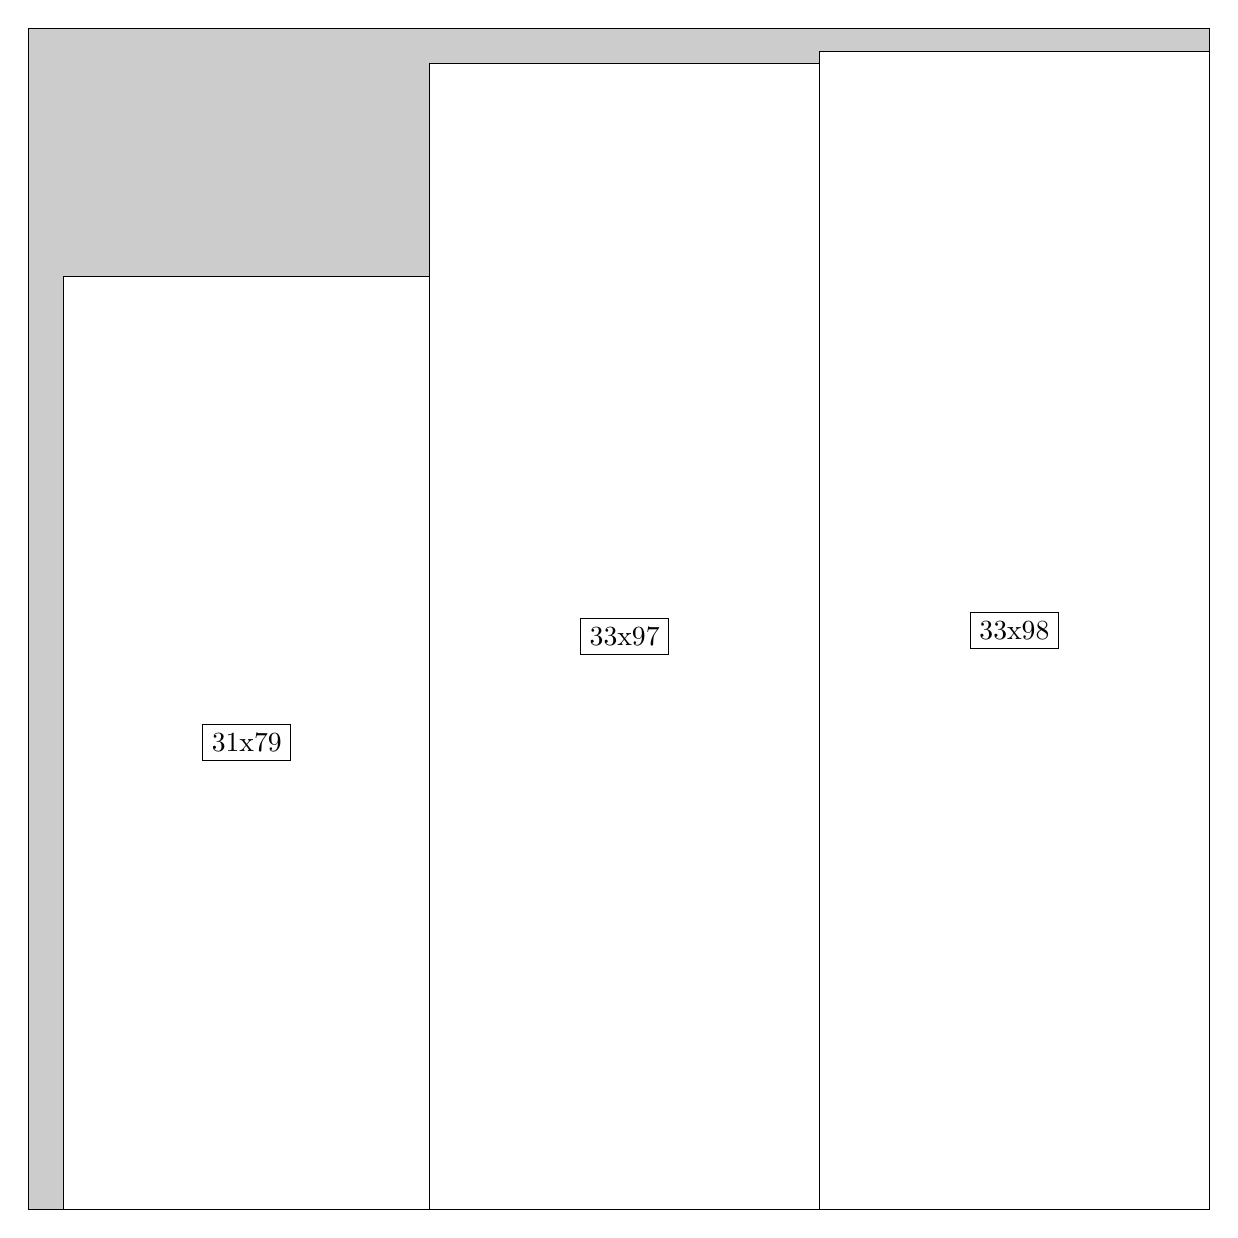
\begin{tikzpicture}[shorten >=1pt,scale=1.0,every node/.style={scale=1.0},->]
\tikzstyle{vertex}=[circle,fill=black!25,minimum size=14pt,inner sep=0pt]
\filldraw[fill=gray!40!white, draw=black] (0,0) rectangle (15.0,15.0);
\foreach \name/\x/\y/\w/\h in {33x98/10.049999999999999/0.0/4.95/14.7,33x97/5.1/0.0/4.95/14.549999999999999,31x79/0.44999999999999996/0.0/4.6499999999999995/11.85}
\filldraw[fill=white!40!white, draw=black] (\x,\y) rectangle node[draw] (\name) {\name} ++(\w,\h);
\end{tikzpicture}


w =33 , h =98 , x =67 , y =0 , v =3234
\par
w =33 , h =97 , x =34 , y =0 , v =3201
\par
w =31 , h =79 , x =3 , y =0 , v =2449
\par
\newpage


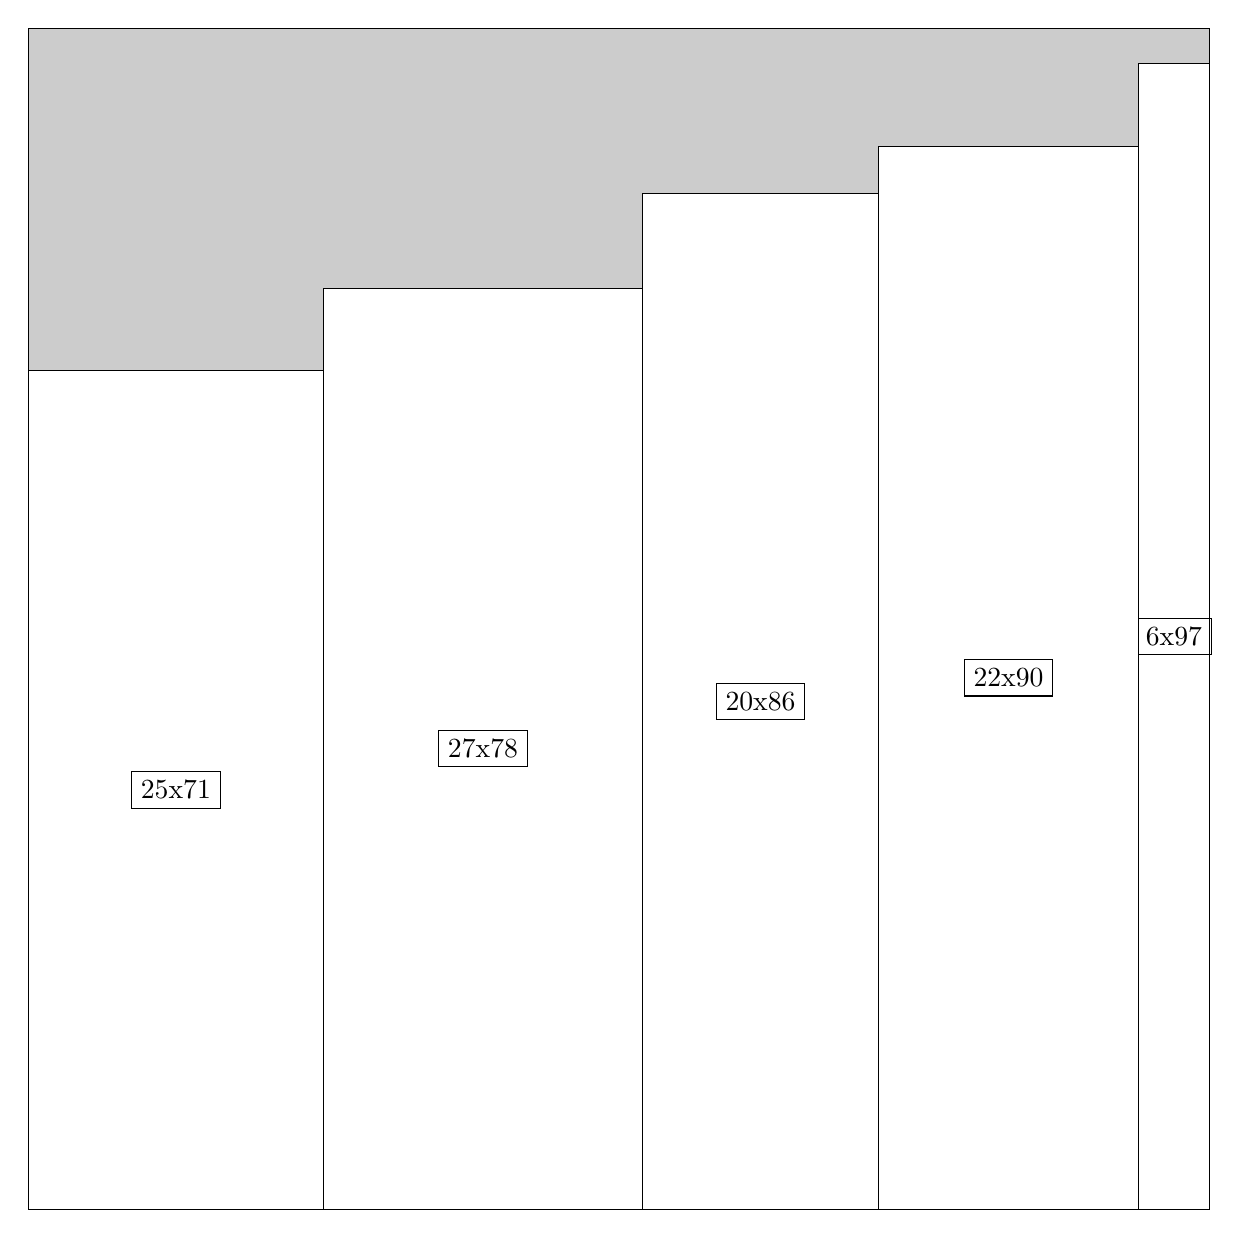
\begin{tikzpicture}[shorten >=1pt,scale=1.0,every node/.style={scale=1.0},->]
\tikzstyle{vertex}=[circle,fill=black!25,minimum size=14pt,inner sep=0pt]
\filldraw[fill=gray!40!white, draw=black] (0,0) rectangle (15.0,15.0);
\foreach \name/\x/\y/\w/\h in {6x97/14.1/0.0/0.8999999999999999/14.549999999999999,22x90/10.799999999999999/0.0/3.3/13.5,20x86/7.8/0.0/3.0/12.9,27x78/3.75/0.0/4.05/11.7,25x71/0.0/0.0/3.75/10.65}
\filldraw[fill=white!40!white, draw=black] (\x,\y) rectangle node[draw] (\name) {\name} ++(\w,\h);
\end{tikzpicture}


w =6 , h =97 , x =94 , y =0 , v =582
\par
w =22 , h =90 , x =72 , y =0 , v =1980
\par
w =20 , h =86 , x =52 , y =0 , v =1720
\par
w =27 , h =78 , x =25 , y =0 , v =2106
\par
w =25 , h =71 , x =0 , y =0 , v =1775
\par
\newpage


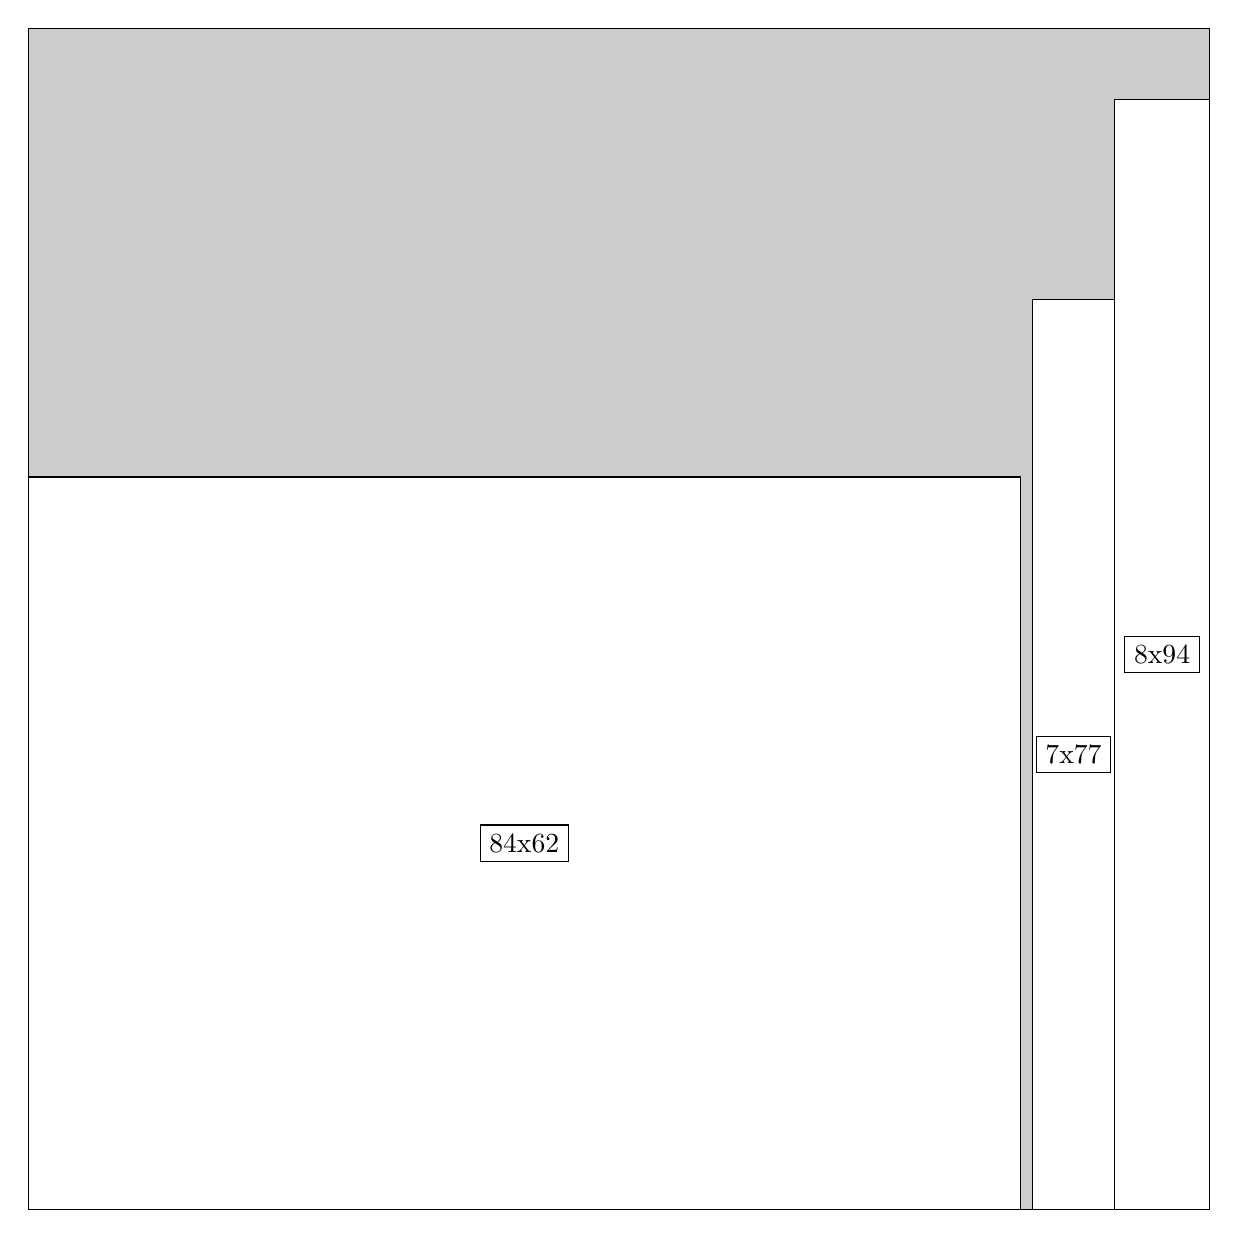
\begin{tikzpicture}[shorten >=1pt,scale=1.0,every node/.style={scale=1.0},->]
\tikzstyle{vertex}=[circle,fill=black!25,minimum size=14pt,inner sep=0pt]
\filldraw[fill=gray!40!white, draw=black] (0,0) rectangle (15.0,15.0);
\foreach \name/\x/\y/\w/\h in {8x94/13.799999999999999/0.0/1.2/14.1,7x77/12.75/0.0/1.05/11.549999999999999,84x62/0.0/0.0/12.6/9.299999999999999}
\filldraw[fill=white!40!white, draw=black] (\x,\y) rectangle node[draw] (\name) {\name} ++(\w,\h);
\end{tikzpicture}


w =8 , h =94 , x =92 , y =0 , v =752
\par
w =7 , h =77 , x =85 , y =0 , v =539
\par
w =84 , h =62 , x =0 , y =0 , v =5208
\par
\newpage


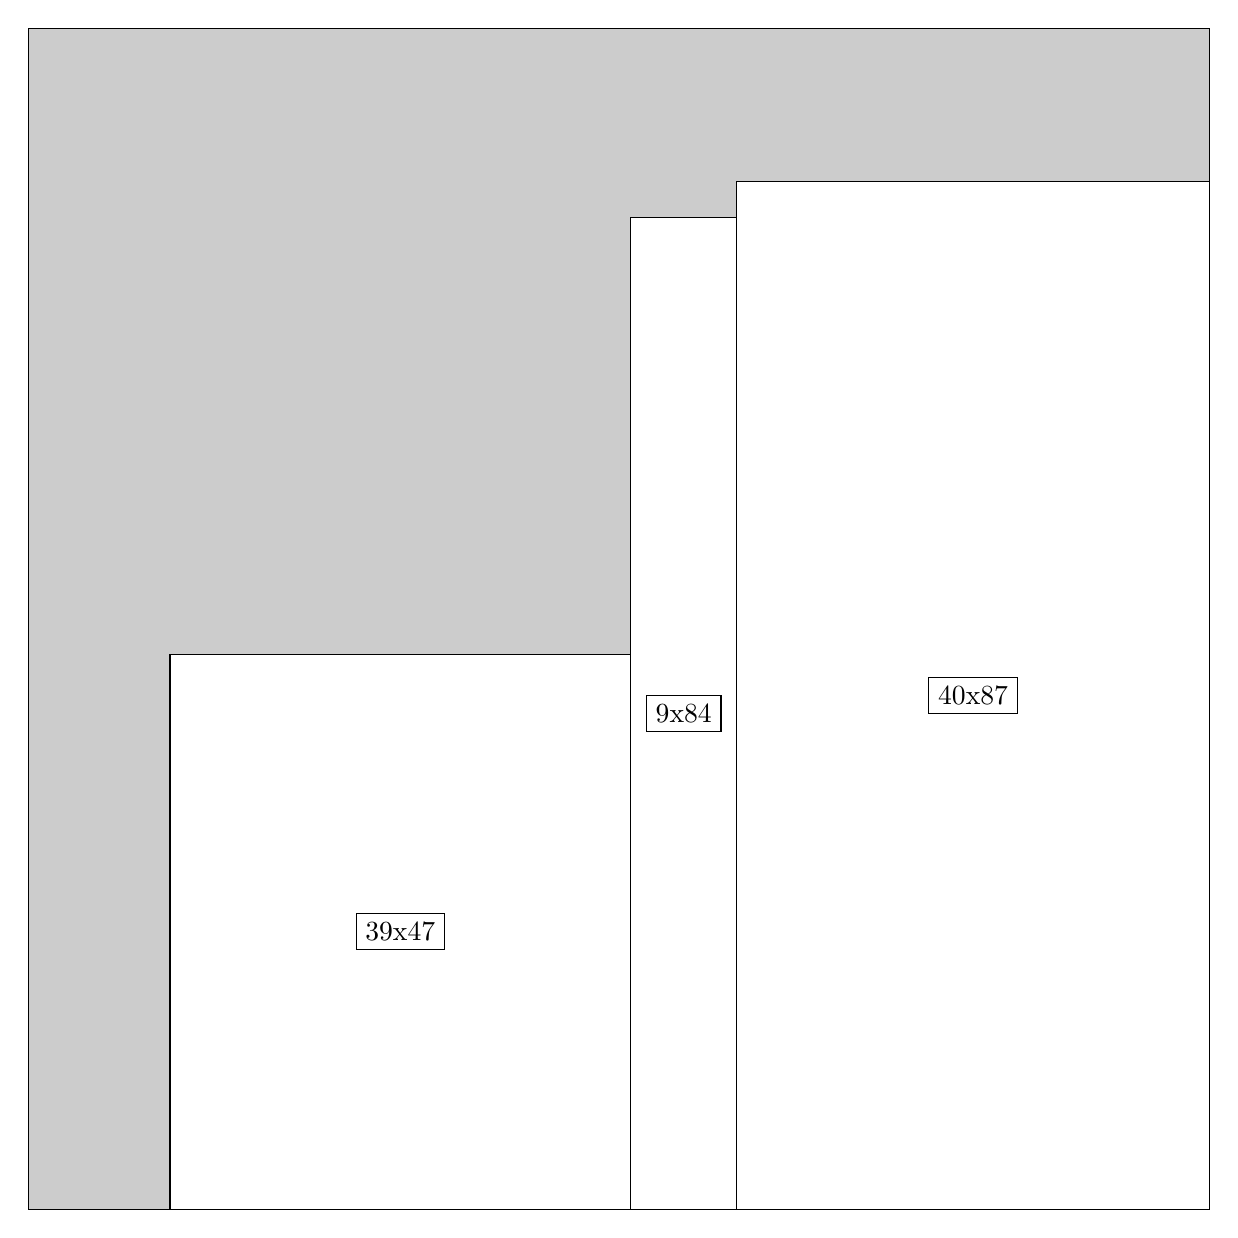
\begin{tikzpicture}[shorten >=1pt,scale=1.0,every node/.style={scale=1.0},->]
\tikzstyle{vertex}=[circle,fill=black!25,minimum size=14pt,inner sep=0pt]
\filldraw[fill=gray!40!white, draw=black] (0,0) rectangle (15.0,15.0);
\foreach \name/\x/\y/\w/\h in {40x87/9.0/0.0/6.0/13.049999999999999,9x84/7.6499999999999995/0.0/1.3499999999999999/12.6,39x47/1.7999999999999998/0.0/5.85/7.05}
\filldraw[fill=white!40!white, draw=black] (\x,\y) rectangle node[draw] (\name) {\name} ++(\w,\h);
\end{tikzpicture}


w =40 , h =87 , x =60 , y =0 , v =3480
\par
w =9 , h =84 , x =51 , y =0 , v =756
\par
w =39 , h =47 , x =12 , y =0 , v =1833
\par
\newpage


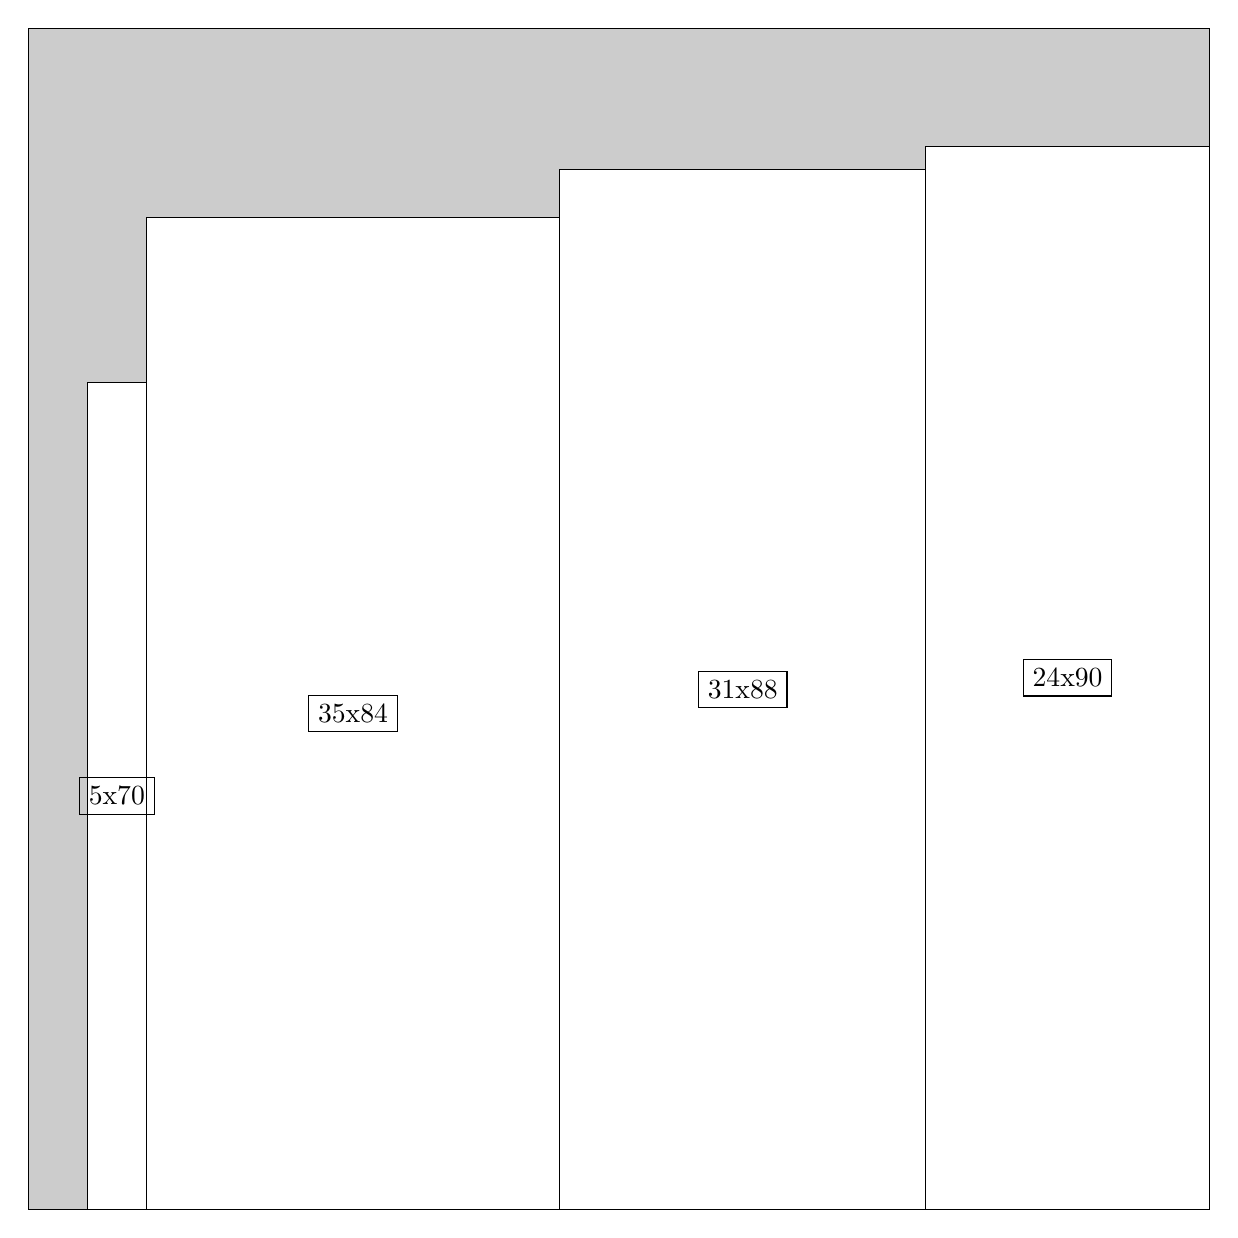
\begin{tikzpicture}[shorten >=1pt,scale=1.0,every node/.style={scale=1.0},->]
\tikzstyle{vertex}=[circle,fill=black!25,minimum size=14pt,inner sep=0pt]
\filldraw[fill=gray!40!white, draw=black] (0,0) rectangle (15.0,15.0);
\foreach \name/\x/\y/\w/\h in {24x90/11.4/0.0/3.5999999999999996/13.5,31x88/6.75/0.0/4.6499999999999995/13.2,35x84/1.5/0.0/5.25/12.6,5x70/0.75/0.0/0.75/10.5}
\filldraw[fill=white!40!white, draw=black] (\x,\y) rectangle node[draw] (\name) {\name} ++(\w,\h);
\end{tikzpicture}


w =24 , h =90 , x =76 , y =0 , v =2160
\par
w =31 , h =88 , x =45 , y =0 , v =2728
\par
w =35 , h =84 , x =10 , y =0 , v =2940
\par
w =5 , h =70 , x =5 , y =0 , v =350
\par
\newpage


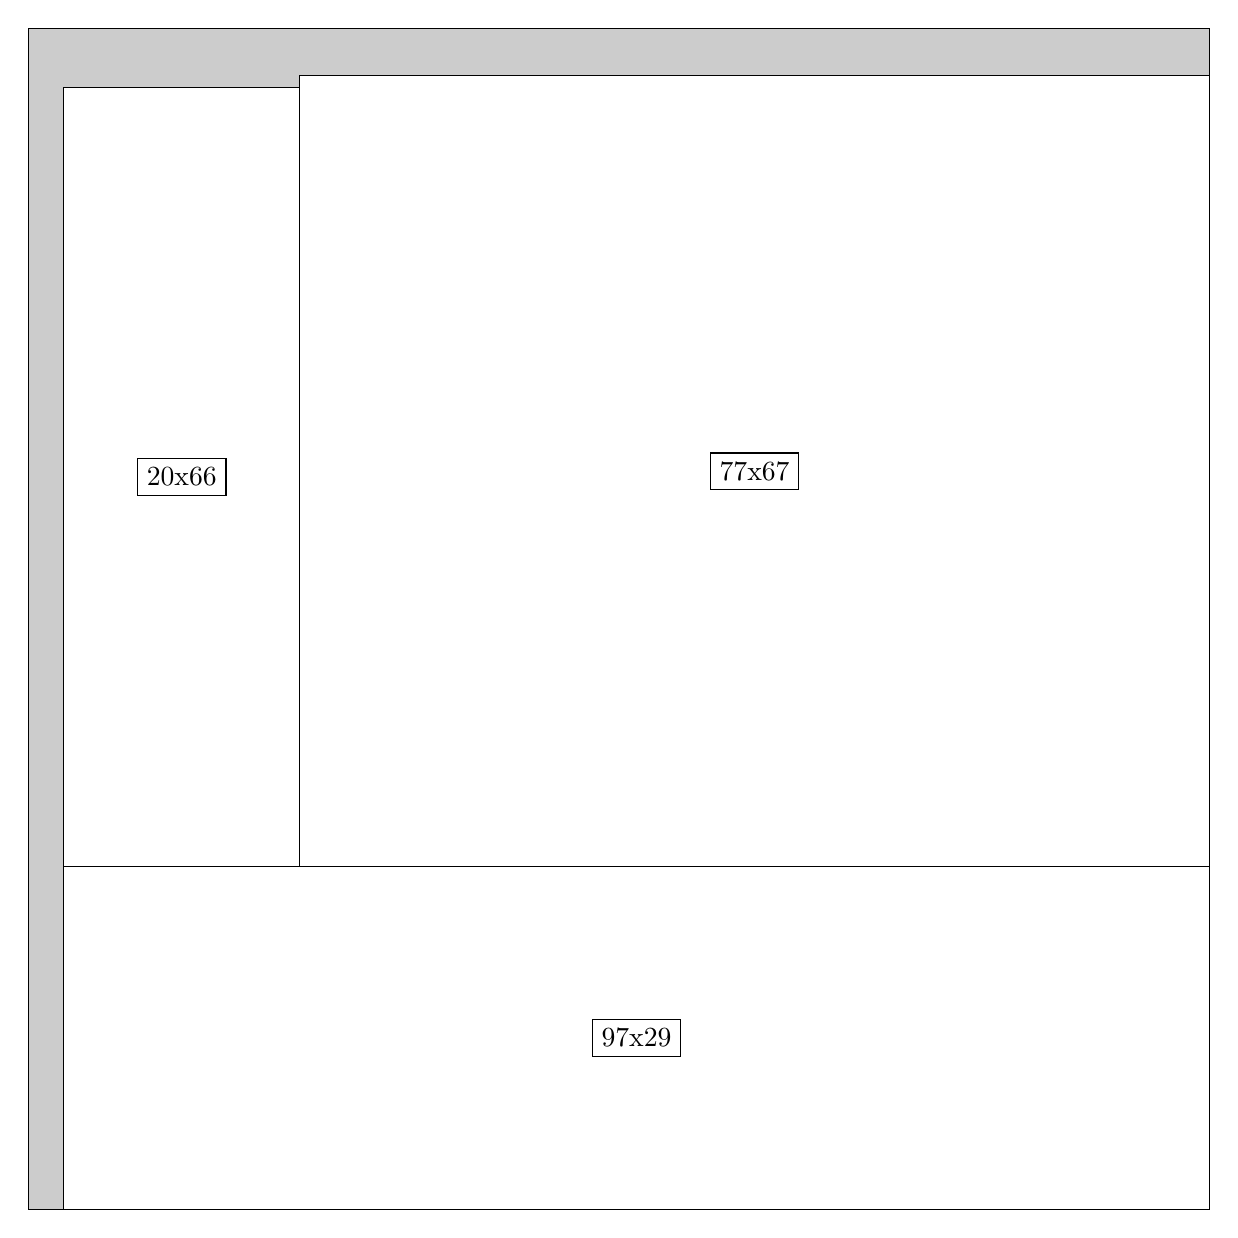
\begin{tikzpicture}[shorten >=1pt,scale=1.0,every node/.style={scale=1.0},->]
\tikzstyle{vertex}=[circle,fill=black!25,minimum size=14pt,inner sep=0pt]
\filldraw[fill=gray!40!white, draw=black] (0,0) rectangle (15.0,15.0);
\foreach \name/\x/\y/\w/\h in {97x29/0.44999999999999996/0.0/14.549999999999999/4.35,77x67/3.4499999999999997/4.35/11.549999999999999/10.049999999999999,20x66/0.44999999999999996/4.35/3.0/9.9}
\filldraw[fill=white!40!white, draw=black] (\x,\y) rectangle node[draw] (\name) {\name} ++(\w,\h);
\end{tikzpicture}


w =97 , h =29 , x =3 , y =0 , v =2813
\par
w =77 , h =67 , x =23 , y =29 , v =5159
\par
w =20 , h =66 , x =3 , y =29 , v =1320
\par
\newpage


\end{document}